\documentclass[11pt,reqno]{amsart}
\usepackage{amssymb}
\usepackage[utf8]{inputenc}
\usepackage{tikz}
\usetikzlibrary{arrows.meta}
\usetikzlibrary{shapes.geometric}
\usetikzlibrary{patterns}
\usetikzlibrary{calc,scopes}
\usetikzlibrary{backgrounds}

\begin{document}

    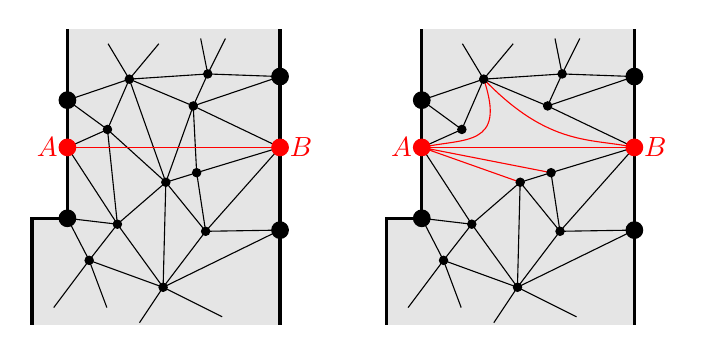
\begin{tikzpicture}[>=stealth,scale=1.5]
    	\coordinate (A) at (0.3,1.6);
    	\coordinate (B) at (2.1,1.6);
    	\coordinate (C) at (0.3,1);
    	\coordinate (D) at (0.3,2.0);
    	\coordinate (E) at (2.1,0.9);
    	\coordinate (F) at (2.1,2.2);
    	\coordinate (K) at (0.723, 0.950);
    	\coordinate (L) at (0.484, 0.644);
    	\coordinate (M) at (1.133, 1.305);
    	\coordinate (N) at (1.365, 1.951);
    	\coordinate (O) at (0.824, 2.178);
    	\coordinate (P) at (0.639, 1.752);
    	\coordinate (Q) at (1.394, 1.386);
    	\coordinate (R) at (1.47, 0.890);
    	\coordinate (S) at (1.488, 2.222);
    	\coordinate (T) at (1.11, 0.416);

        % surface on the left
        \filldraw[gray!20!white] (0,0.1) -- (0,1) -- (0.3, 1) -- (0.3,2.6)--(2.1,2.6)--(2.1,0.1)--cycle;
        \draw[very thick] (0,0.1) -- (0,1) -- (0.3, 1) -- (0.3,2.6);
       	\draw[very thick] (2.1,0.1) -- (2.1,2.6);
       	
       	\draw (D) -- (O) -- (P) -- (D);
       	\draw (O) -- (M) -- (P);
       	\draw (O) -- (S) -- (N) -- (F) -- (S);
       	\draw (O) -- (N) -- (M) -- (Q) -- (N) -- (B) -- (Q);
       	\draw (M) -- (K) -- (P) -- (A) -- (K) -- (C) -- (L) -- (K) -- (T) -- (L);
       	\draw (T) -- (M) -- (R) -- (T) -- (E) -- (R) -- (Q);
       	\draw (B) -- (R);
       	
       	\draw 
       		($(L) + (-0.3,-0.4)$) -- (L) -- ($(L) + (0.15,-0.4)$)
       		($(T) + (-0.2,-0.3)$) -- (T) -- ($(T) + (0.5,-0.25)$)
       		($(S) + (-0.06,0.3)$) -- (S) -- ($(S) + (0.15,0.3)$)
       		($(O) + (-0.18,0.3)$) -- (O) -- ($(O) + (0.25,0.3)$);
       	\foreach \p in {(K),(L),(M),(N),(O),(P),(Q),(R),(S),(T)}
			\filldraw \p circle (1pt);
       	\filldraw[red] 
       		(A) circle (2pt)
       		(B) circle (2pt);
       	\filldraw
       		(C) circle (2pt)
       		(D) circle (2pt)
       		(E) circle (2pt)
       		(F) circle (2pt);
       	\draw[red] (A) -- (B);
       	\draw[red] 
       		(A) node[left]{$A$}
       		(B) node[right]{$B$};
       	
       	%surface on the right
       	\filldraw[gray!20!white] (3,0.1) -- (3,1) -- (3.3, 1) -- (3.3,2.6)--(5.1,2.6)--(5.1,0.1)--cycle;
       	\draw[very thick] (0+3,0.1) -- (0+3,1) -- (0.3+3, 1) -- (0.3+3,2.6);
       	\draw[very thick] (2.1+3,0.1) -- (2.1+3,2.6);
       	
       	\draw ($(D)+(3,0)$) -- ($(O)+(3,0)$) -- ($(P)+(3,0)$) -- ($(D)+(3,0)$);
       	\draw ($(O)+(3,0)$) -- ($(S)+(3,0)$) -- ($(N)+(3,0)$) -- ($(F)+(3,0)$) -- ($(S)+(3,0)$);
       	\draw ($(O)+(3,0)$) -- ($(N)+(3,0)$);
       	\draw ($(M)+(3,0)$) -- ($(Q)+(3,0)$);
       	\draw ($(N)+(3,0)$) -- ($(B)+(3,0)$) -- ($(Q)+(3,0)$);
       	\draw ($(M)+(3,0)$) -- ($(K)+(3,0)$) -- ($(A)+(3,0)$) -- ($(P)+(3,0)$);
       	\draw ($(K)+(3,0)$) -- ($(C)+(3,0)$) -- ($(L)+(3,0)$) -- ($(K)+(3,0)$) -- ($(T)+(3,0)$) -- ($(L)+(3,0)$);
       	\draw ($(T)+(3,0)$) -- ($(M)+(3,0)$) -- ($(R)+(3,0)$) -- ($(T)+(3,0)$) -- ($(E)+(3,0)$) -- ($(R)+(3,0)$) -- ($(Q)+(3,0)$);
       	\draw ($(B)+(3,0)$) -- ($(R)+(3,0)$);
       	\draw 
       	($(L) + (3-0.3,-0.4)$) -- ($(L)+(3,0)$) -- ($(L) + (3.15,-0.4)$)
       	($(T) + (3-0.2,-0.3)$) -- ($(T)+(3,0)$) -- ($(T) + (3.5,-0.25)$)
       	($(S) + (3-0.06,0.3)$) -- ($(S)+(3,0)$) -- ($(S) + (3.15,0.3)$)
       	($(O) + (3-0.18,0.3)$) -- ($(O)+(3,0)$) -- ($(O) + (3.25,0.3)$);
       	
       	\coordinate (AA) at ($(A) + (3,0)$);
       	\coordinate (BB) at ($(B)+(3,0)$);
       	\coordinate (KK) at ($(K)+(3,0)$);
       	\coordinate (LL) at ($(L)+(3,0)$);
       	\coordinate (MM) at ($(M)+(3,0)$);
       	\coordinate (NN) at ($(N)+(3,0)$);
       	\coordinate (OO) at ($(O)+(3,0)$);
       	\coordinate (PP) at ($(P)+(3,0)$);
       	\coordinate (QQ) at ($(Q)+(3,0)$);
       	\coordinate (RR) at ($(R)+(3,0)$);
       	\coordinate (SS) at ($(S)+(3,0)$);
       	\coordinate (TT) at ($(T)+(3,0)$);
       	
       	\draw[red] 
       		(QQ) -- (AA) -- (MM);
       	\draw[red]
       		(AA) ..controls ($(AA)!0.2!(BB) + (0,0.08)$) and ($(AA)!0.4!(BB)$) ..(OO)
       		(BB) ..controls ($(AA)!0.8!(BB) + (0,0.08)$) and ($(AA)!0.6!(BB)$) ..(OO);
       	\foreach \p in {(KK),(LL),(MM),(NN),(OO),(PP),(QQ),(RR),(SS),(TT)}
       	\filldraw \p circle (1pt);
       	\filldraw[red] 
       	($(A)+(3,0)$) circle (2pt)
       	($(B)+(3,0)$) circle (2pt);
       	\filldraw
       	($(C)+(3,0)$) circle (2pt)
       	($(D)+(3,0)$) circle (2pt)
       	($(E)+(3,0)$) circle (2pt)
       	($(F)+(3,0)$) circle (2pt);
       	\draw[red] ($(A)+(3,0)$) -- ($(B)+(3,0)$);
       	\draw[red] 
       	($(A)+(3,0)$) node[left]{$A$}
       	($(B)+(3,0)$) node[right]{$B$};
    \end{tikzpicture}

\end{document}